\begin{tikzpicture}[auto, node distance=3.5cm, auto, >=latex']
     % We start by placing the blocks
     \node [input, name=input] {};
     \node [block, right of=input] (dac) {DAC};
     \node [block, right of=dac] (system) {$G(s)$};
     \node [block, right of=system] (adc) {ADC};
     \node [output, name=output, right of=adc] {};

     % Once the nodes are placed, connecting them is easy. 
     \draw [draw,->] (input) -- node {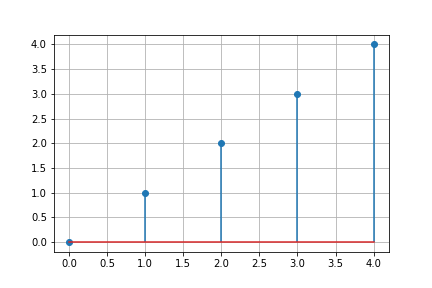
\includegraphics[width=100px]{img/xk.png}} (dac);
     \draw [->] (dac) -- node {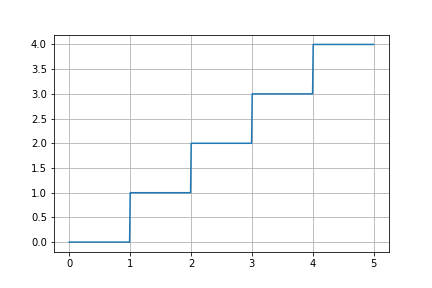
\includegraphics[width=100px]{img/dac.png}} (system);
     \draw [->] (system) -- node {$Y(s)$} (adc);
     \draw [->] (adc) -- node {$Y(z)$} (output);
\end{tikzpicture}